%!TEX root = ./aistats_2019_sketchmcmc.tex

\section{Experiments}

\begin{figure}
\subfigure[]{
	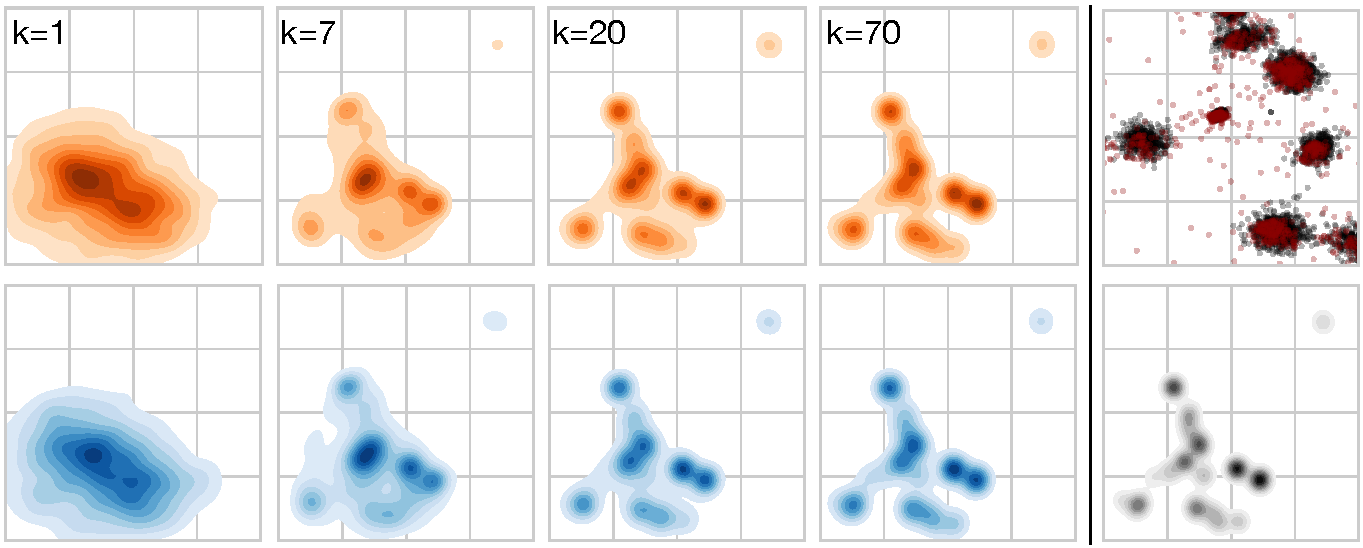
\includegraphics[width=0.65\columnwidth]{gmm_iter.pdf}
	\label{fig:toy_example}
} \hfill
\subfigure[]{
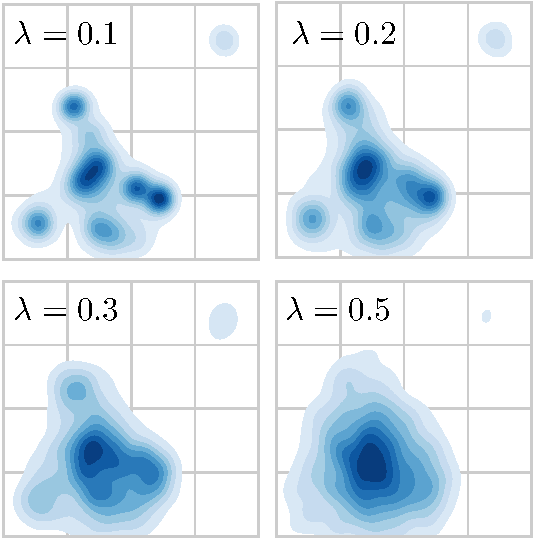
\includegraphics[width=0.255\columnwidth]{gmm_reg.pdf}
\label{fig:lambda_supp}
 }
 % \vspace{-\baselineskip}
\caption{a) \textbf{Left:} Distribution of particles (contour plots) during the estimation (top) and prediction (bottom) stages. \textbf{Right:} (top) Close-up of some generated particles in red superimposed with data points in black. (bottom) Target distribution. b) Influence of the regularization parameter~$\lambda$. }
\end{figure}

%
In this section, we evaluate the SWF algorithm on both synthetic and real data settings. In all cases, the initial distribution $\mu_0$ is selected as the standard Gaussian distribution on $\R^d$, we take $Q=100$ quantiles, which proved sufficient to approximate the quantile functions, and we have observed that $N=3000$ particles are sufficient. We provide an example implementation in \supp.


\begin{figure}
% \begin{wrapfigure}{R}{0.40\textwidth}
% \vspace{-10pt}
\begin{centering}
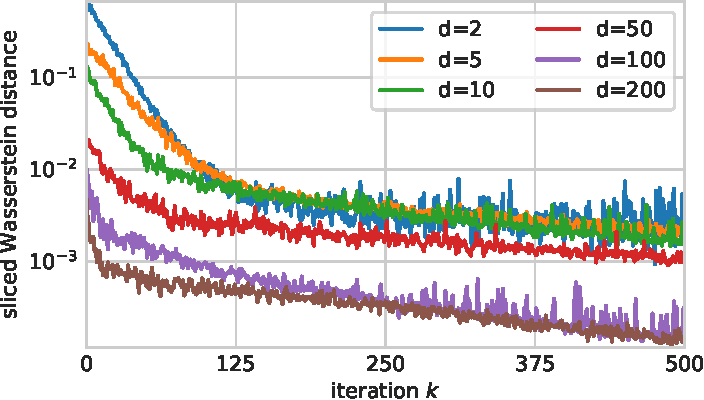
\includegraphics[width=0.40\columnwidth]{SW2_cost-crop.pdf}
\par\end{centering}
\caption{Approximately computed $\SW$ between the output $\bar{\mu}_{k}^{N}$ and data distribution $\nu$ in the GMM model for different data dimensions $d$.
\label{fig:toy_sw}}
% \vspace{-10pt}
\end{figure}
% \end{wrapfigure}
% \textbf{Gaussian Mixture Model: }
\subsection{Gaussian Mixture Model }
We perform the first set of experiments on synthetic data where we consider a standard Gaussian mixture model (GMM).
%
We set the number of the mixture components to $20$ and for each component we randomly draw the weight, covariance matrix and the centroid. We make sure that the centroids are sufficiently distant from each other in order to make the problem more challenging. Given the model parameters, we generate $P=50000$ data samples in each experiment.


In our first experiment, we set $d=2$ for visualization purposes and illustrate the general behavior of the algorithm. Figure~\ref{fig:toy_example} shows the evolution of the particles through the iterations. Here, we set $N_\theta=30$, $h=1$, and $\lambda=10^{-4}$.
%
We observe that the empirical distribution of the particles converges rapidly to the target distribution. Furthermore, we can see that the QF, $F^{-1}_{\theta^*_\#\bar{\mu}_{kh}^{N}}$ that is computed with one set of particles (so-called the \textit{estimation} stage) can be perfectly re-used for new unseen particles in a subsequent \textit{prediction} stage. In both cases, we observe two remarkable outcomes: (i) Even when some modes are isolated from the others, SWF is able to capture them successfully and we never observe a mode collapse. This is due to the OT nature of the procedure. (ii) The generated particles do not collapse on the data points, thanks to the entropy regularization.

In our second experiment, we investigate the effect of the level of the regularization. We use the same setting as the previous experiment, whereas we differ the value of $\lambda$ and run the algorithm for sufficiently many iterations. As we can observe from Figure~\ref{fig:lambda_supp}, the distribution of the particles becomes more spread with increasing $\lambda$. This is due to the increment of the entropy, as expected.



We also illustrate the behavior of the algorithm for varying dimensionality $d$. Since visualizing the results becomes non-trivial for large $d$, in this experiment we directly monitor the (approximately computed) $\SW$ distance between the distribution of the particles and the data distribution. Even though minimizing this distance is not the real objective of our method, arguably, it is still a good proxy for understanding the convergence behavior.
%
Figure~\ref{fig:toy_sw} illustrates the results. We observe that, for all choices of $d$, we see a steady decrease in the cost for all runs, which is in line with our theory. We also observe that the magnitude of $\SW$ decreases as $d$ increases. This outcome can be explained by the fact that $\SW = {\cal O}(d^{-1/2}\W)$ (cf.\ \cite{bonnotte2013unidimensional}).








\subsection{Experiments on real data}
% \label{sub:real_data}

% \textbf{Experiments on real data: }
%
In a second set of experiments, we test the SWF algorithm on two real datasets. (i) The traditional MNIST dataset that contains 70K binary images corresponding to different digits (of size $28 \times 28$, i.e.\ $d = 784$). (ii) The recently proposed FashionMNIST dataset \cite{xiao2017fashion}, that contains $50000$ gray-scale images. All images were interpolated as $64\times 64$, yielding $d=4096$. This dataset is advocated as more challenging than MNIST.

Our goal in these experiments is to capture the structure of the data distribution such that the particles that are generated by the algorithm will be samples from this unknown data distribution. In these experiments, we set $\lambda=10^{-6}$ and $N_\theta=200$. We will present visual results for qualitative inspection. %More results with higher resolution are given in \supp.

Figures~\ref{fig:mnist} and \ref{fig:fashionmnist}, show that SWF is able to generate samples from the datasets in a few thousand iterations. We can observe that, the generated samples for the MNIST dataset are considerably accurate. For the FashionMNIST dataset, the samples capture the prominent features of the training samples; the generated samples take the form of various clothings along the iterations. By considering that SWF only requires the projections of the data points, in a way, all these samples are generated without seeing the actual dataset.




Another important advantage of SWF is its low computational requirements. The whole experiment on the FashionMNIST requires around $1$ hour of computational time on the CPU of a standard laptop computer, to be compared with the significant resource requirements of the current IGM methods.








\begin{figure}[t]
\centering
\subfigure[MNIST]{
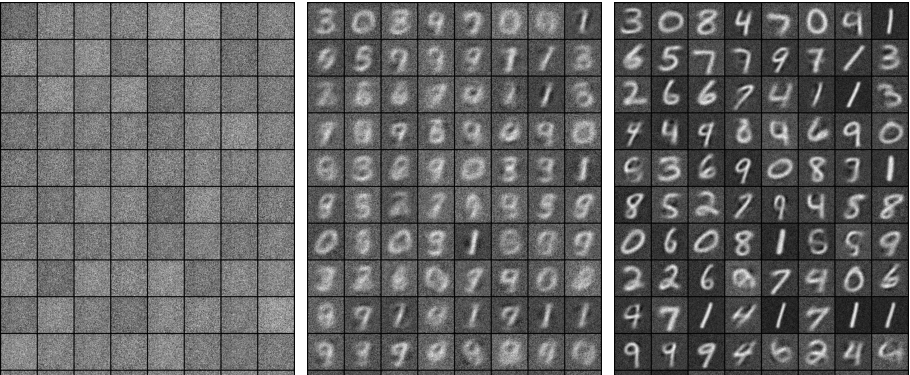
\includegraphics[width=0.41\columnwidth]{mnist.pdf}
\label{fig:mnist}
}\hfill
\subfigure[Fashion MNIST]{
\includegraphics[width=0.55\columnwidth]{fmnist2.pdf}
\label{fig:fashionmnist}
}
% \vspace{-10pt}
\caption{The evolution of the particles through $15000$ iterations on different datasets.}
% \vspace{-10pt}
\end{figure}










